%!TEX program=xelatex
\documentclass[10pt]{beamer}
\usepackage[UTF8,noindent]{ctexcap}
\usepackage{listings}

\usetheme{metropolis}
\usepackage{appendixnumberbeamer}

\usepackage{booktabs}
\usepackage[scale=2]{ccicons}

\usepackage{pgfplots}
\usepgfplotslibrary{dateplot}

\usepackage{xspace}
\newcommand{\themename}{\textbf{\textsc{metropolis}}\xspace}

\title{解决问题的艺术}
\subtitle{The Art of Problem Solving}
\date{\today}
\author{熊丘桓}
\institute{南京大学微软俱乐部}
% \titlegraphic{\hfill
\includegraphics[height=1.5cm]{logo.pdf}}

\begin{document}

\maketitle

\begin{frame}{目录}
    \setbeamertemplate{section in toc}[sections numbered]
    \tableofcontents[hideallsubsections]
\end{frame}


\begin{frame}[fragile]{Self Introduction}
    熊丘桓,软件学院2020级本科生。

    现任微软俱乐部技术部副部长。

    任软件学院C程序设计基础助教、开甲书院朋辈导师(以及招生志愿者)。

    深谙“解决问题”艺术。
\end{frame}

\section{提问之前:初探疑云}

\begin{frame}[fragile]{提问之前:初探疑云}
    在您准备要通过电子邮件、新闻群组或者聊天室提出技术问题前,请先做到以下事情:
    \begin{itemize}
        \item 他山之石:尝试在搜索引擎、论坛的旧文章中搜索答案。
        \item 官方预备:尝试阅读手册、常见问题文件(FAQ)以找到答案。
        \item 自力更生:尝试自己检查或试验以找到答案;如果您是程序开发者,请尝试阅读源代码以找到答案。
        \item 向你身边的强者朋友打听以找到答案。
    \end{itemize}

    当你提出问题的时候,请先表明你已经做了上述的努力;这将有助于树立你并不是一个不劳而获且浪费别人的时间的提问者。如果你能一并表达在做了上述努力的过程中所学到的东西会更好,因为我们更乐于回答那些表现出能从答案中学习的人的问题。
\end{frame}

\begin{frame}[fragile]{尝试上网搜索}
    内事问百度(但很多广告扰乱搜索结果)

    外事、技术问谷歌(重点来了,怎么访问?

    必应介于二者之间

    Stack Exchange Community

    \begin{itemize}
        \item Super User 通用的电脑问题
        \item Stack Overflow 程序有关问题
        \item Server Fault 服务器和网管相关问题
    \end{itemize}
    博客:博客园(cnblogs,近期访问困难),CSDN,开源中国

    工具轮子:GITHUB,码云

    Linux相关:askubuntu,archwiki

    此外:知乎,思否(SegmentFault),阿里云,腾讯云
\end{frame}

\begin{frame}[fragile]{尝试上网搜索}
    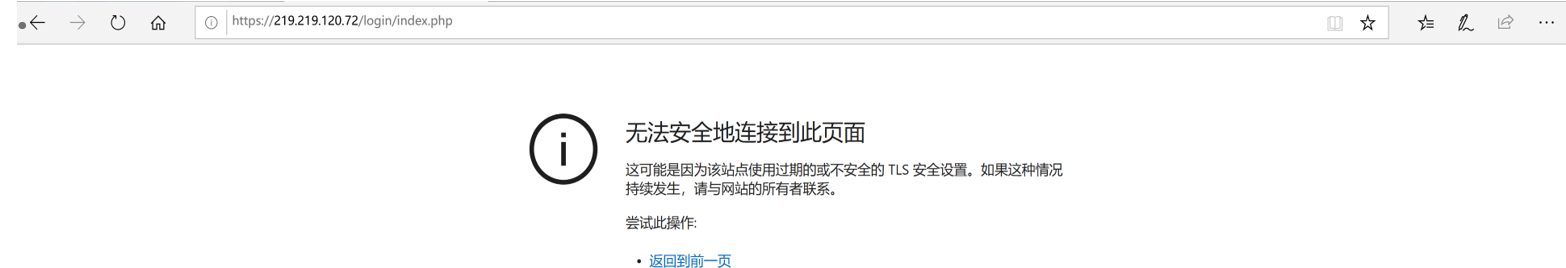
\includegraphics[width=\textwidth]{pic/error-1.png}

    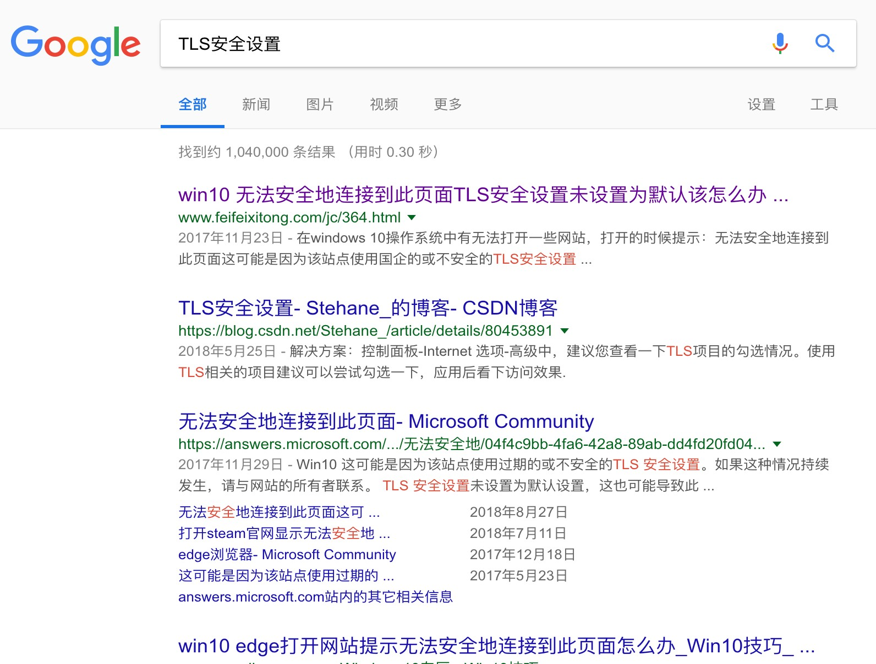
\includegraphics[width=0.7\textwidth]{pic/sol-1.png}
\end{frame}

\begin{frame}[fragile]{尝试自己检查或试验以找到答案}
    查bug原因:
    \begin{itemize}
        \item 断点调试,看具体变量
              \begin{itemize}
                  \item Visual Studio
                  \item JetBrains全家桶,有学生免费账户:https://www.jetbrains.com/student/
              \end{itemize}
        \item print/alert/assert大法
        \item Machine is ALWAYS RIGHT!
    \end{itemize}
    确认了bug原因:
    \begin{itemize}
        \item 复制关键信息,上网搜索。如“ArrayOutOfBoundException”
    \end{itemize}
\end{frame}

\begin{frame}[fragile]{提问之前:初探疑云}
    尝试在你准备提问的论坛的旧文章中搜索答案

    尝试阅读手册(Manual)以找到答案

    尝试阅读FAQ(Frequently Asked Questions)以找到答案

    向你身边的dalao打听以找到答案
\end{frame}

\section{当提问时:切中肯綮}

\begin{frame}{当提问时:切中肯綮}
    拋出的一个技术问题最终是否能得到有用的回答,往往与你提问和追问的方式有较大关联

    黑客们(或大佬们)喜爱有挑战性的问题,或者能激发他们思维的好问题;黑客们有着对那些不愿思考、或者在发问前不做他们该做的事的人的蔑视

    能立刻得到快速并有效答案的最好方法,就是聪明、自信、有解决问题的思路,只是偶尔在特定的问题上需要获得一点帮助
\end{frame}

\begin{frame}[fragile]{慎选提问的论坛}
    小心选择你要提问的场合,不要:

    \begin{itemize}
        \item 在与主题不合的论坛上贴出你的问题
        \item 在探讨进阶技术问题的论坛张贴非常初级的问题;反之亦然
        \item 在太多的不同群组上重复转贴同样的问题(cross-post)
        \item 向既非熟人也没有义务解决你问题的人发送私人邮件
    \end{itemize}

    用Google找到与你遭遇到困难的软硬件问题最相关的网站。通常那儿都有FAQ、邮件列表及相关说明文件的链接

    提问前在群组或邮件列表的历史记录中搜索与问题相关的关键词

    依照个人经验,大部分的问题都可以通过搜索得到指引或解决
\end{frame}

\begin{frame}[fragile]{提问}
    准备好你的问题,草率的发问只能得到草率的回答
    \begin{quote}
        “我在 Google 中搜过下列句子但没有找到什么有用的东西”
    \end{quote}

    表现出只要有人能指个正确方向,你就有完成它的能力和决心
    \begin{quote}
        好:“我的这个例子里缺了什么”,“我应该检查什么地方”

        坏:“请把我需要的确切的过程贴出来”
    \end{quote}

    表现出只要有人能指个正确方向,你就有完成它的能力和决心


    不要自以为够格(entitled to)得到答案,你并没有。你没有为这种服务支付任何报酬。你将会是靠提出有内涵的、有思维激励作用的问题自己去挣到一个答案
\end{frame}

\begin{frame}[fragile]{简洁的标题}
    坏标题:“帮帮忙”、“跪求”、“急”、“救命啊”

    使用“物体-偏差”(object - deviation)式描述的标题。在物体部分指出是哪一个或哪一组东西有问题,在差异部分则描述与期望的行为不一致的地方

    \begin{quote}
        好:XXX-Y 型号的鼠标光标,在某牌显卡 MV1005 芯片组环境下会变形

        有助于你组织对问题的细致思考:是什么被影响了? 仅仅是鼠标光标或者还有其它图形?只在 XXX的 鼠标中出现?或只是出现在 Y 版中? 是针对某牌显卡芯片组?或者只是其中的 MV1005 型号?
    \end{quote}

\end{frame}

\begin{frame}[fragile]{描述问题}
    首先应该通过初筛确定问题,至少确定一个范围,比如:版本兼容的问题,环境依赖的问题或代码某段出错等等

    之后用尽量简明准确的语言进行描述,例如:在使用xxx版本的navicat时,无法连接localhost中的MySQL数据库。使用的MySql版本为xxx

    注意礼貌与表达感谢,如:在提问后跟  谢谢大神/抱拳了老铁/thanks a lot 之类的话(分场合搭配),以及跟一些有趣的表情包
\end{frame}

\begin{frame}[fragile]{Stack Overflow}
    Stack Exchange community 已成为回答技术及其他问题的主要渠道

    \begin{enumerate}
        \item 先在 Google 搜索。有很高的机率某人已经问了一个类似的问题,而且 Stack Exchange 往往会是搜索结果中最前面几个
        \item 如果Google上找不到,到Stack Overflow里搜索。使用tag来narrow down搜索结果。tag一般是编程语言,操作系统和库等
        \item 再提问。提问时使用tag
    \end{enumerate}

    在国内,可能不得不使用低配版Google -- Bing

    谷歌学术用不了?-- Microft Academic
\end{frame}

\begin{frame}[fragile]{Stack Overflow}
    搜索样例:编程语言等各种tag + 在做什么事情中遇到了问题 + 错误信息

    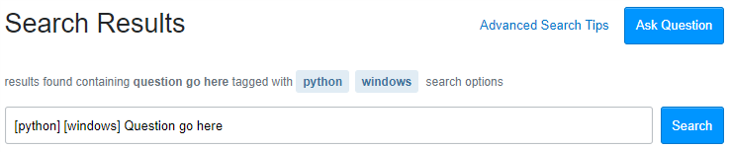
\includegraphics[width=\textwidth]{pic/search-results.png}

    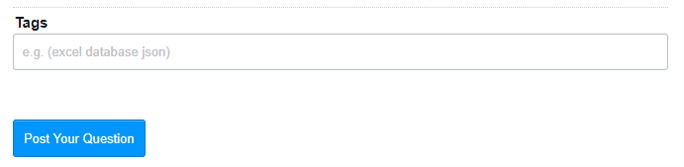
\includegraphics[width=\textwidth]{pic/tags.png}
\end{frame}

\begin{frame}[fragile]{Stack Overflow}
    
\includegraphics[width=\textwidth]{pic/stack-overflow.png}

    需要魔法,否则访问困难

    Stack Overflow网站的jQuery需要跨域调用Google JavaScript API,网站顶部总会提示“Stack Overflow requires external JavaScript from another domain, which is blocked or failed to load” ,Google“躺枪”后Stack Overflow也被拉下水了

    注意到如果你只是临时看看的话,可以用AdBlocker之类的软件禁用此类JavaScript达成访问效果!
\end{frame}

\section{解读答案:拨云见日}

\begin{frame}[fragile]{RTFM 和 STFW}
    有一个古老而神圣的传统:如果你收到RTFM的回应,回答者认为你应该去读手册(Read The Friendly Manual);如果你收到STFW的回应,回答者认为你应该到网上搜索(Search The Friendly Web)。更温和一点的说法是“Google 是你的朋友”!

    类似于我们的:本群已和百度、高德达成深度合作……

    你又丢人了
\end{frame}

\begin{frame}[fragile]{如果还是搞不懂}
    别立刻要求对方解释。像你以前试着自己解决问题时那样(利用手册,FAQ,网络,身边的高手),先试着去搞懂他的回应。如果你真的需要对方解释,记得表现出你已经从中学到了点什么!
\end{frame}

\section{科研问题:学海无涯}

\begin{frame}[fragile]{做好文献检索}
    在开始一个研究时,最难的往往是入手和确定方向。这时就需要查找已有的相关研究结果,了解最新进展以及目前所需的工作。

    通过阅读文献还可以学习到一些适用于此问题的数学方法、软/硬件等的知识,省去了自己查找、踩坑的用时

    看到别人的优秀成果时也能激励自己,一方面说明这个方向是可以做出一些有价值的东西的,另一方面也会激发出自己探索的热情,见贤思齐

    尽量确保你在校园网环境下,当你看到“南京大学”/ “南京大学图书馆”的时候,你就可以放心了!
\end{frame}

\begin{frame}[fragile]{常用检索方式}
    南大图书馆数据库

    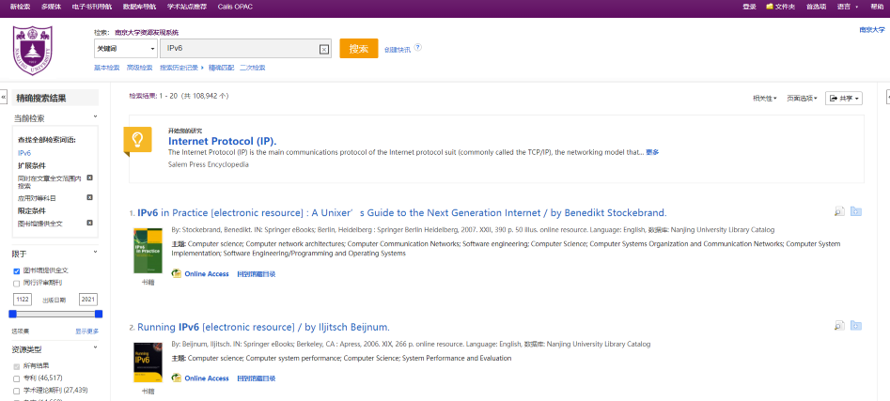
\includegraphics[width=\textwidth]{pic/NJU-library.png}
\end{frame}

\begin{frame}[fragile]{常用检索方式}
    知网 - https://cnki.net/

    注意需要在校园网环境下访问(p.nju.edu.cn)

    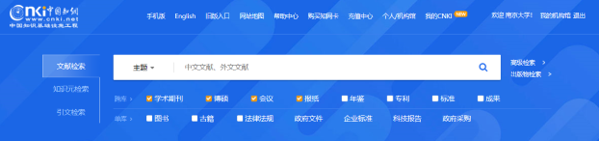
\includegraphics[width=\textwidth]{pic/CNKI.png}

    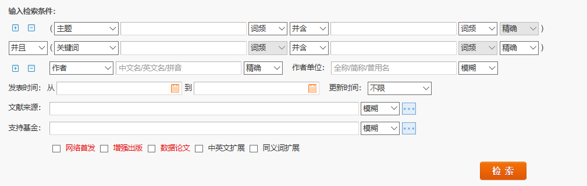
\includegraphics[width=\textwidth]{pic/CNKI-2.png}

\end{frame}

\begin{frame}[fragile]{常用检索方式}
    万方 - http://wanfangdata.com.cn/index.html

    注意需要在校园网环境下访问(p.nju.edu.cn)

    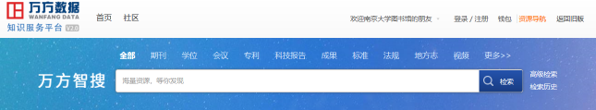
\includegraphics[width=\textwidth]{pic/Wanfang-1.png}

    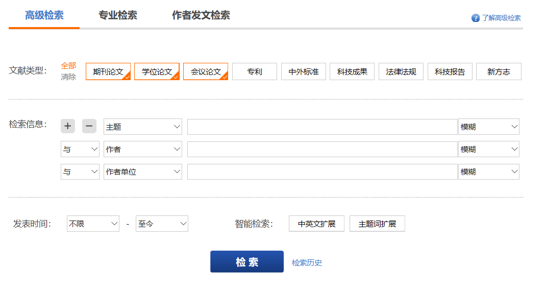
\includegraphics[width=\textwidth]{pic/Wanfang-2.png}
\end{frame}

\begin{frame}[fragile]{常用检索方式}
    Web Of Science

    注意需要在校园网环境下访问(p.nju.edu.cn)

    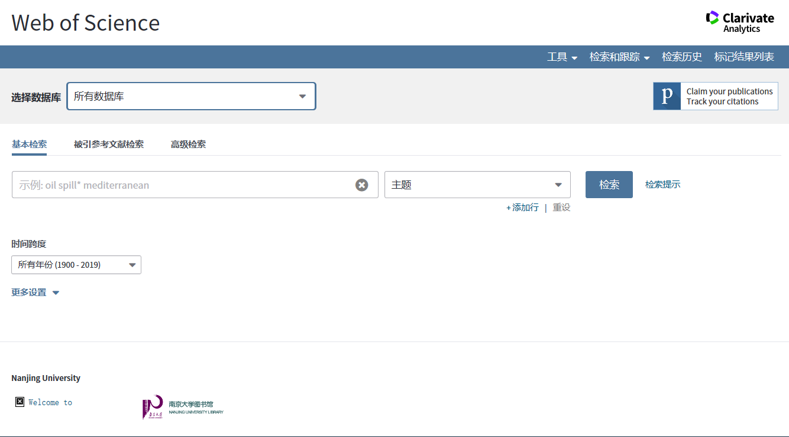
\includegraphics[width=\textwidth]{pic/WebOfScience.png}
\end{frame}

\begin{frame}[fragile]{常用检索方式}
    如果Web Of Science没有版权 请找ACM - https://dl.acm.org/dl.cfm

    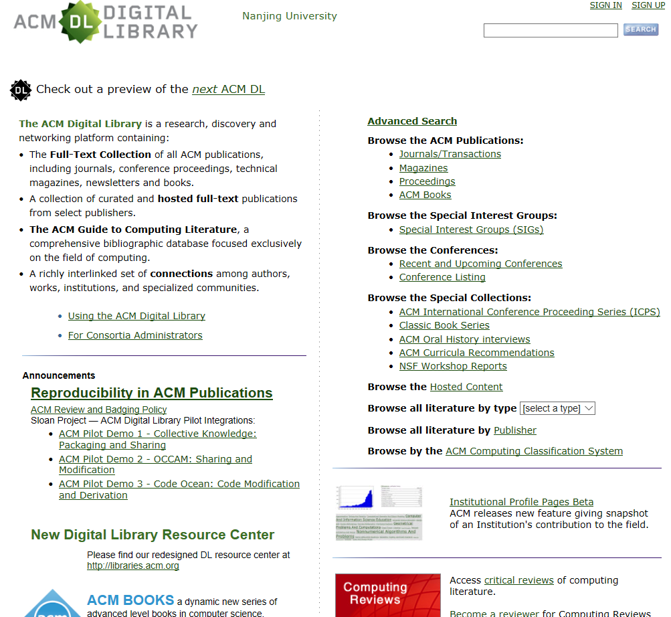
\includegraphics[width=0.7\textwidth]{pic/ACM.png}
\end{frame}

\begin{frame}[fragile]{查找论文的方式}
    \begin{enumerate}
        \item 按标题查找(一般搜的都是知名论文,比如 《can machines think》)
        \item 随缘查找,得到结果后点击—按被引数排序,找到经典结果;点击—按时间排序,找到最新成果(但也许不那么可靠)
        \item 在随缘查找的基础上找到几篇比较靠谱的文章(逻辑清晰,论述有据,方法有效,被引率高,发表在可信期刊上等等),从文末的引用里再调几篇合适的论文。这些一般来说也是比较可靠的文章。
    \end{enumerate}
\end{frame}

\begin{frame}[fragile]{必备品}
    \begin{itemize}
        \item 一款好用的markdown软件(推荐typora)
        \item 微软必应词典/有道词典等翻译工具
        \item 思路清晰的大脑
        \item 集中的注意力(反正我看一会英文就会困)
        \item 我南的Adobe Acrobat DC 高级多功能pdf阅读器(丝滑+多功能)
    \end{itemize}
\end{frame}

\begin{frame}[standout]

    The Art of Problem Solving

    Do it yourself, and BELIEVE in yourself!

    NJUMSC传统艺能

    主讲人:熊丘桓
    
\end{frame}

\end{document}
